\documentclass[../../main.tex]{subfiles}

\begin{document}


\begin{longtable}{| p{.20\textwidth} | p{.80\textwidth} |} 
\hline
    Kratak opis & Klijent želi da se prijavi za program obuke kako bi dobio licencu za trenera.  \\ 
\hline    
    Učesnici &
    \begin{enumerate}
        \item Klijent
        \item Recepcioner
    \end{enumerate}\\
\hline
   Preduslovi &
   \begin{enumerate}
        \item Sistem je u funkciji
        \item Klijent je registrovan (tj. član je teretane)
        \item Recepcioner je prijavljen na sistem
    \end{enumerate}\\
\hline  
    Postuslovi & 
    \begin{enumerate}
        \item Klijent je prijavljen za program obuke
    \end{enumerate} \\
\hline
    Osnovni tok & 
    \begin{enumerate}
        \item Klijent dolazi na recepciju.
        \item Recepcioner ukratko informiše klijenta o svakom programu obuke koji se održava.
        \item Klijent govori recepcioneru koji program želi da pohađa.
        \item Recepcioner štampa formular za prijavu na taj program.
        \item Recepcioner predaje formular klijentu.
        \item Klijent popunjava formular.
        \item Klijent vraća recepcioneru popunjen formular.
        \item Recepcioner proverava da li su popunjena sva obavezna polja u formularu.
        \item Recepcioner govori klijentu koja dokumenta je još potrebno da mu da.
        \item Klijent daje potrebna dokumenta.
        \item Recepcioner uzima dokumenta.
        \item Recepcioner odlaže dokumenta i popunjen formular na mesto odakle će ih uzeti neko iz uprave teretane ko je zadužen za program obuke.
        \item Recepcioner u deo sistem koji je posvećen prijavi uživo unosi osnovne informacije o klijentu - ime, prezime, broj članske karte, koliko dugo trenira i šta trenira.
        \item Recepcioner čekira polje u formularu kojim potvrđuje da je dokumenta ostavio na odgovarajućem mestu.
        \item Sistem šalje potvrdu da je prijava uspešno sačuvana.
        \item Recepcioner obaveštava klijenta da je prijava uspešna.
        \item Klijent odlazi.
    \end{enumerate}\\
\hline
    Alternativni tokovi & 
    \begin{itemize}
        \item[A8] Nisu popunjena sva obavezna polja. Recepcioner vraća klijentu formular da ih popuni. Slučaj upotrebe se nastavlja u koraku 7.
        \item[A10] Klijent nema sva potrebna dokumenta. Recepcioner privremeno čuva popunjen formular i govori klijentu da donese dokumenta sledeći put kad bude dolazio. Slučaj upotrebe se završava. 
    \end{itemize} \\
\hline
    Podtokovi & /\\
\hline
    Specijalni zahtevi & /\\
\hline
    Dodatne informacije &
    \begin{enumerate}
        \item Informacije koje se unose u formular su ime i prezime klijenta, broj članske karte, gde je i koliko dugo trenirao pre nego što je došao u ovu teretanu i slično.
        \item Dokumenta koje klijent prilaže su: potvrde da je osvojio nagrade na nekim takmičenjima ukoliko je učestvovao na takmičenjima; potvrda o tome koliko dugo je član ove teretane; ukoliko je pre trenirao na nekom drugom mestu, potvrda o tome koliko dugo je trenirao tamo.
    \end{enumerate}\\
\hline
\caption{Uživo prijava za program obuke}
\end{longtable}

\begin{figure}[!ht]
\begin{center}
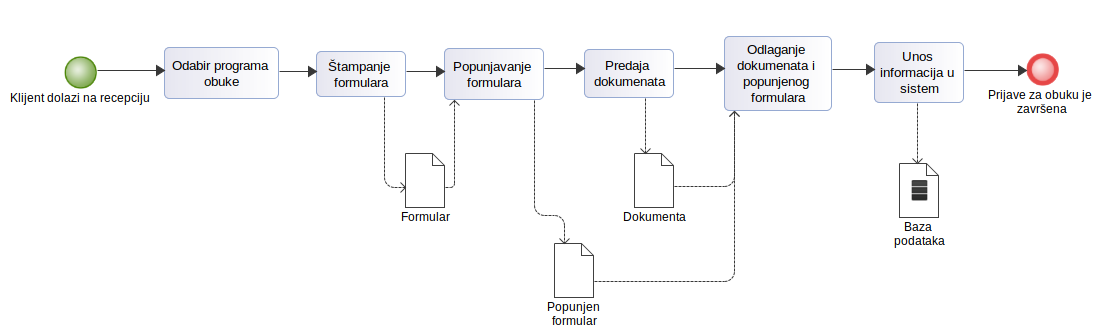
\includegraphics[scale=0.40]{sections/images/bpmn_dijagram_procesa_prijava_za_licencu.png}
\end{center}
\caption{BPMN dijagram procesa za prijavu na program obuke za licencu}
\label{fig:kontekst}
\end{figure}

\newpage
\begin{figure}[!ht]
\begin{center}
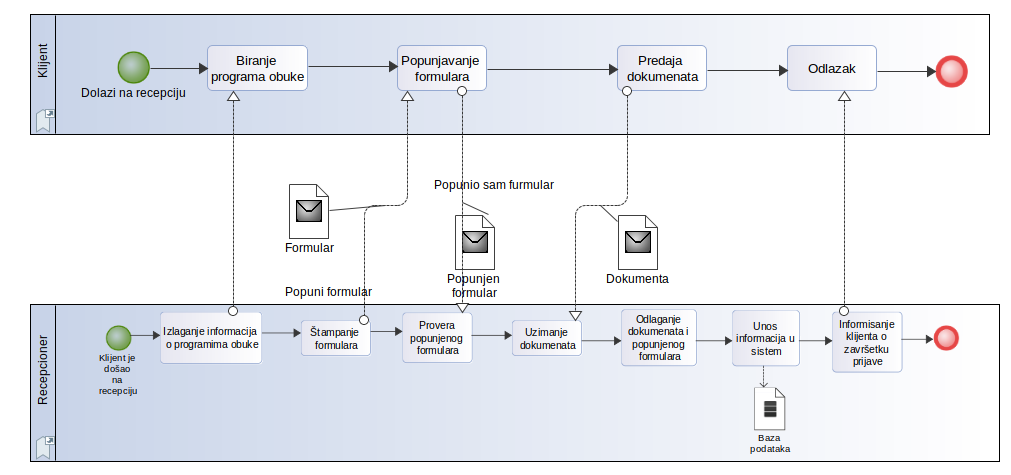
\includegraphics[scale=0.45]{sections/images/bpmn_dijagram_saradnje_prijava_za_licencu.png}
\end{center}
\caption{BPMN dijagram saradnje za prijavu na program obuke za licencu}
\label{fig:kontekst}
\end{figure}

\end{document}